\documentclass{article}

\usepackage{amsmath}
\usepackage{physics}
\usepackage{empheq}
\usepackage{amssymb}
\usepackage{gensymb}
\usepackage{graphicx}
\usepackage{wrapfig}
\usepackage[margin=1.0in]{geometry}

\usepackage[backend=bibtex,style=verbose-note,citepages=suppress]{biblatex}
\addbibresource{hot_tap_weld_report.bib}

\makeatletter
\newcommand{\autocitel}[1]{\autocite{#1}\checknextarg}
\newcommand{\checknextarg}{\@ifnextchar\bgroup{\gobblenextarg}{}}
\newcommand{\gobblenextarg}[1]{$^,$\autocite{#1}\@ifnextchar\bgroup{\gobblenextarg}{}}
\makeatother

\title{Hot Tap Welding Model}
\author{Ravi Kedarasetti}
\date{}

\begin{document}
\maketitle

\section{Problem statement}

Hot tapping \autocitel{twi} (or pressure tapping) is the method of connecting to a "live" pipeline or tank containing a pressurized fluid, without removing the pipe or tank from service. When welding is used to add attachments to a pipeline during hot tapping, the heat transfer around the weld could be a major concern. If the unmelted portion of pipe wall beneath the weld is not thick enough, it might not withstand the pressure of the fluid. In some cases, the excess cooling provided by the flowing liquid could lead to cold cracking of the weld. Thermal models are often used to simulate the heat transfer around the welds to estimate the safe operating ranges for heating rates to prevent burn through and cold cracking\autocitel{bruce2006comparison}.\\  

\begin{wrapfigure}[25]{r}{0.48\textwidth}
	\centering
	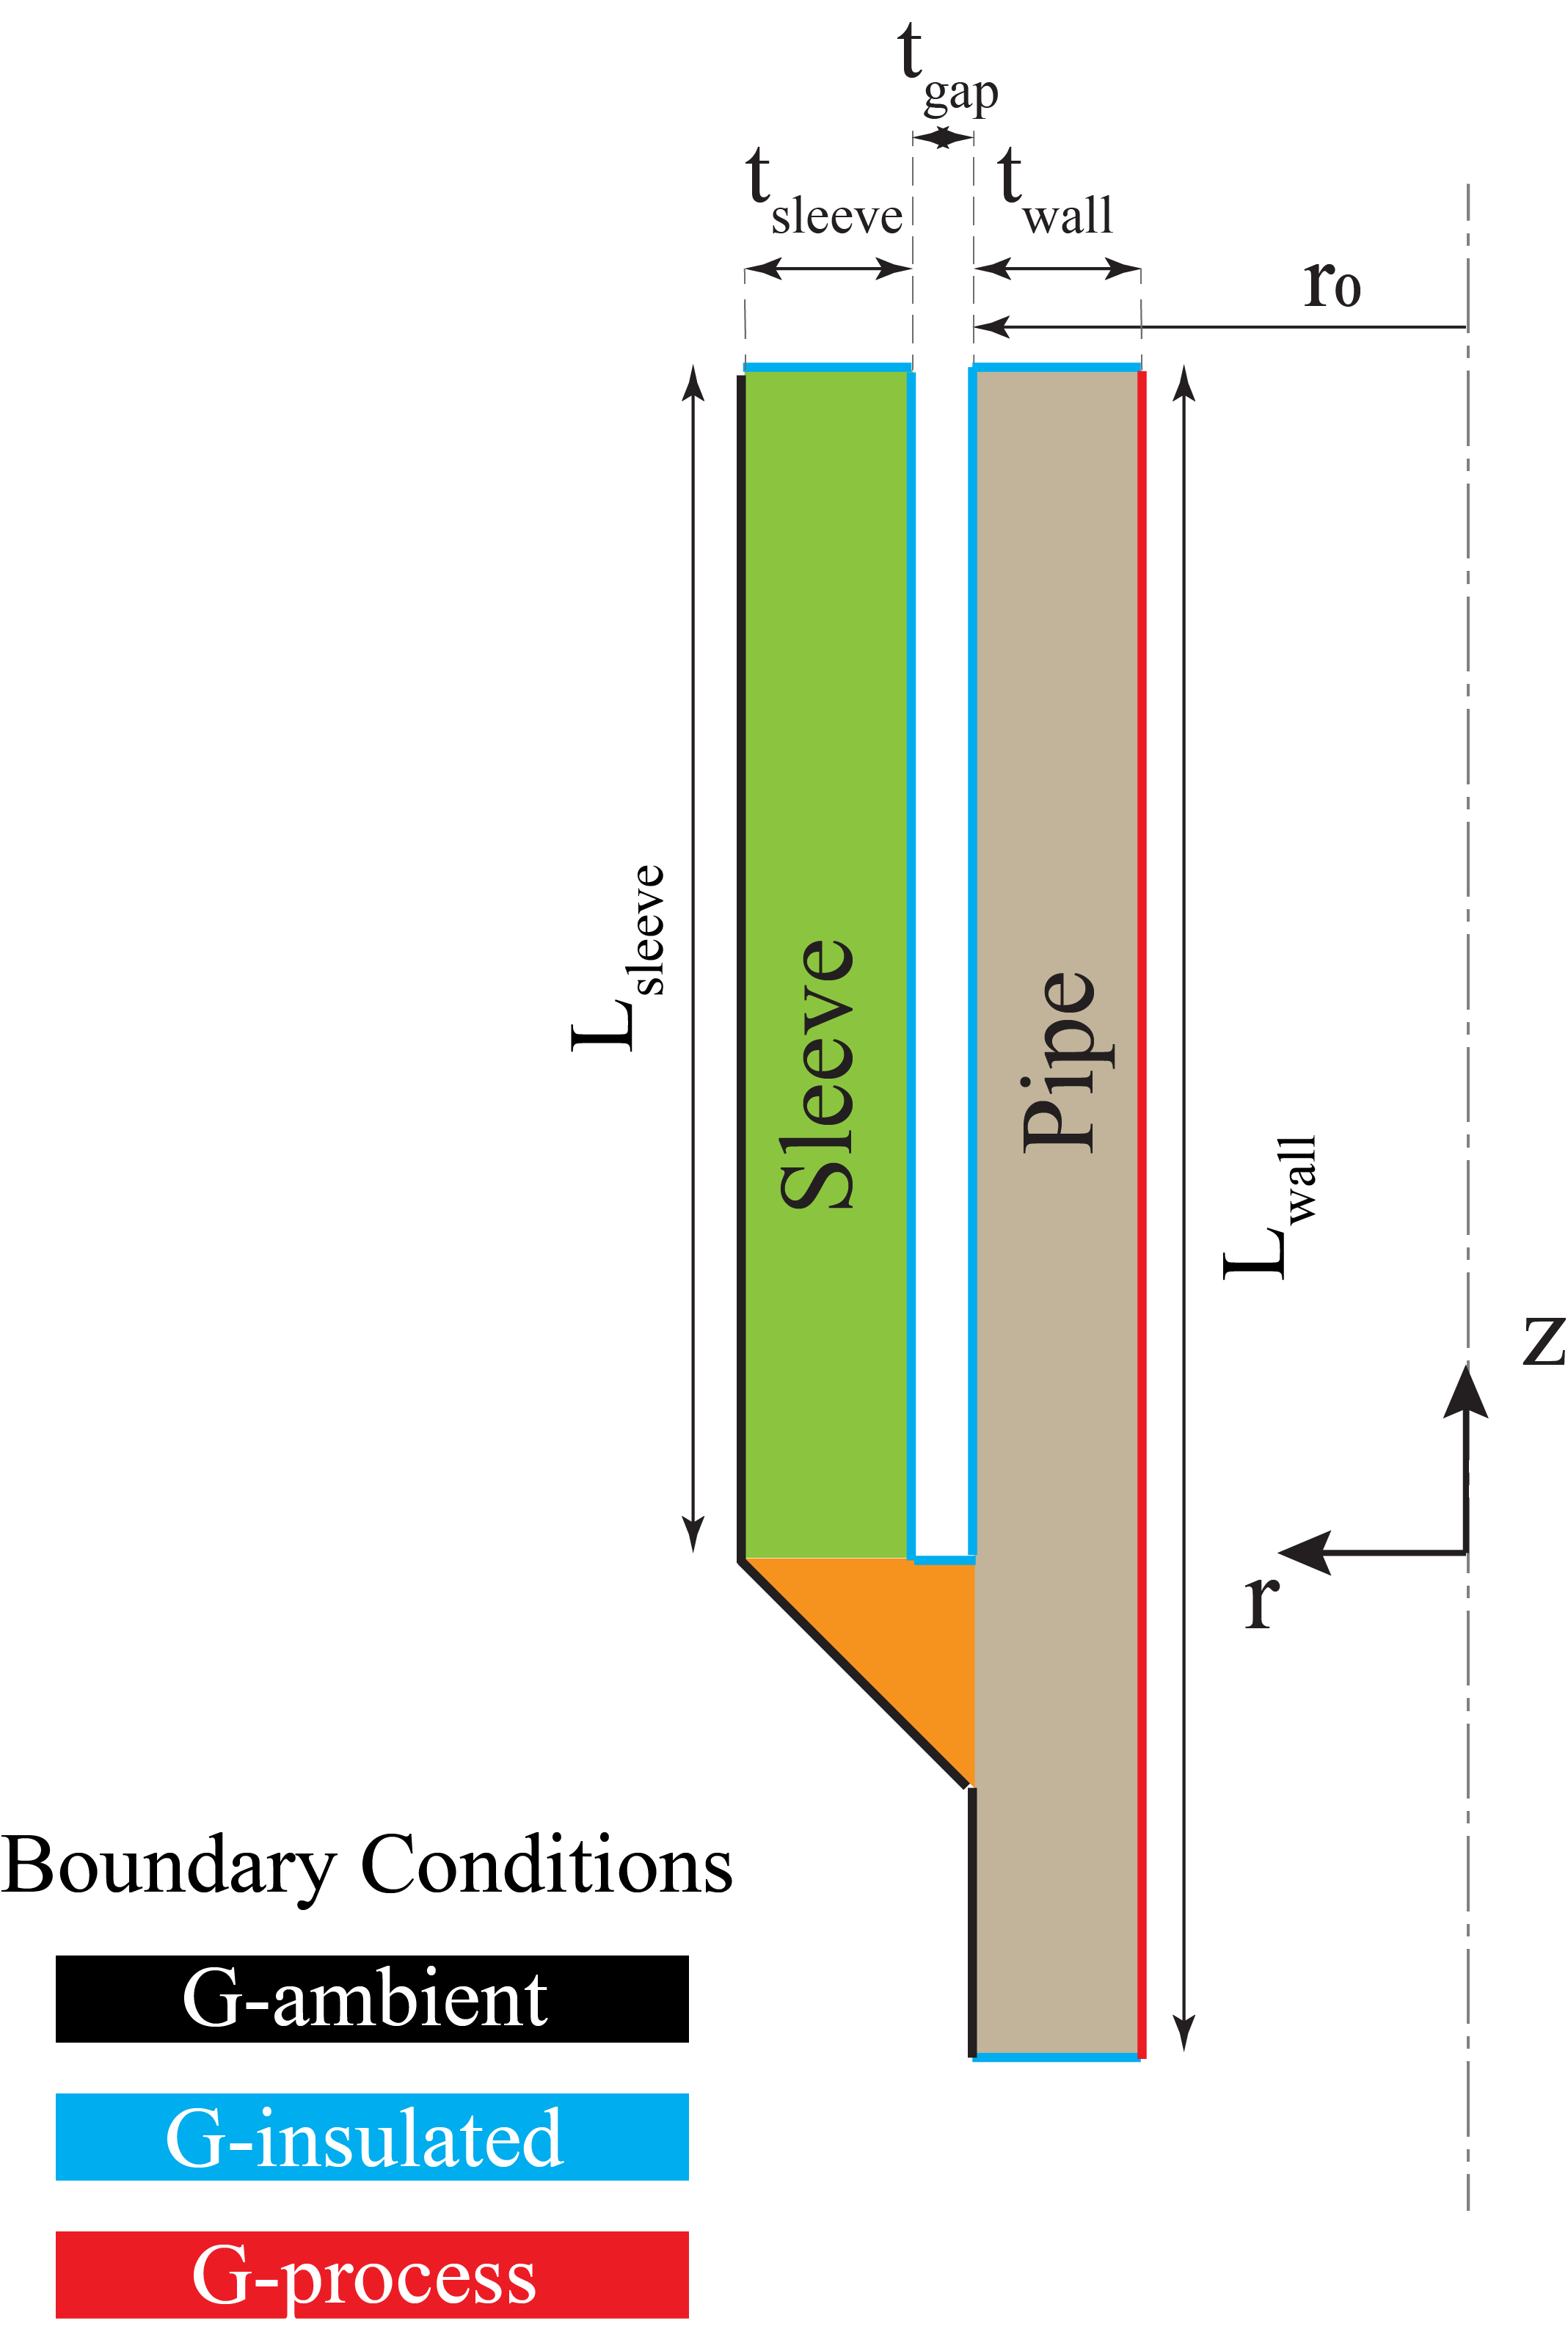
\includegraphics[width=0.46\textwidth]{problem_statement.png}
	\caption{Axisymmetric model showing the pipe (brown), sleeve (green) and weld( orange) geometries and the boundary conditions}
	\label{fig1}
\end{wrapfigure}

 Consider a simplified, axisymmetric thermal model of hot taping process, where a sleeve is welded onto a live pipe carrying fluid. In this problem, a cylindrical stainless steel sleeve of thickness $t_{sleeve}$ and length $L_{sleeve}$ is welded onto a pipe of outer radius $r_0$, wall thickness of $t_{wall}$ and a length of $L_{wall}$, with a small gap of thickness $t_{gap}$ between the wall and the sleeve, as shown in figure \ref{fig1}. The cross section of the weld is assumed to be a right-angled isosceles triangle. The material in the whole model has a mass-density $\rho$, thermal conductivity $\kappa$ and heat capacity $c_p$. During the welding process, heat $f(r,z,t)$ is supplied to the weld. The inner wall of the pipe is in contact with the fluid being transported at temperature $u_p$, while the outer wall of the entire geometry is surrounded by ambient atmosphere at temperature $u_a$ The heat transfer coefficients at the inner and outer walls are $h_p$ and $h_a$ respectively. The surface of the walls facing the gap between the sleeve and the pipe, and the axial ends of the sleeve and the pipe are assumed to be insulated. The boundary conditions are depicted in figure \ref{fig1}. The parameters and their units are presented in table \ref{table:1}. \\ \\
 
\newpage
\begin{table}[h!]
\centering
\begin{tabular}{l|c|c|l}
Parameter & Value & Unit & Description \\
\hline
$t_{sleeve}$ & 0.188 & $in$ & Sleeve thickness \\
$L_{sleeve}$ & $10*t_{sleeve}$ & $in$ & Sleeve Length \\
$t_{wall}$ & $t_{sleeve}$ & $in$ & Pipe wall thickness \\
$L_{wall}$ & $1.5*L_{sleeve}$ & $in$ & Pipe wall length \\
$t_{gap}$ & 0.02 & $in$ & Gap Thickness \\
$t_{weld}$ & $t_{sleeve} + t_{gap}$ & $in$ & Weld height \\
$\rho$ & 0.284 & $lb/in^3$ & mass density \\
$c_p$ & 0.199 & $BTU/lb-F$ & heat capacity \\
$\kappa$ & 31.95 & $BTU/ht-ft-F$ & heat conductivity \\
$u_a$ & 70 & $F$ & Ambient temperature \\
$h_a$ & 9.0 & $BTU/hr-ft^2-F$ & Heat transfer coefficient - ambient \\
$u_p$ & 325 & $F$ & Internal fluid temperature \\
$h_p$ & 48.0 & $BTU/hr-ft^2-F$ & Heat transfer coefficient - Internal fluid \\
$f_{max}$ & 1350 & $BTU/s-in^3$ & maximum heat generated 
\end{tabular}
\caption{Model parameters}
\label{table:1}
\end{table}

\section{Formulation}
\subsection{Strong form}
 This model is based on the linear heat equation. The spatio-temporal evolution of temperature $u$ is governed by equation \ref{heatEqn}, where $\Omega_s$, $\Omega_p$ and $\Omega_w$ are the domains representing the sleeve, pipe and weld respectively. The timecourse of the heat source is defined in equation \ref{heatSource}.
 
\begin{align}
\rho c_p \pdv{u}{t} &= \kappa \laplacian{u} + f(r, z, t) \qquad \qquad in~ \Omega = \Omega_s \cup \Omega_p \cup \Omega_w  \label{heatEqn}   \\
f(r, z, t) &= \begin{cases}
\frac{f_{max}}{2} (1 + \cos{\frac{\pi}{5}(t + 5)}) \qquad & in ~ \Omega_w \\
0  \qquad & in ~  \Omega_s\cup\Omega_p
\end{cases} \label{heatSource}
\end{align}

The boundary conditions are given by equations \ref{gAmb}-\ref{gPro}, where $\Gamma_a$, $\Gamma_i$ and $\Gamma_p$ are the boundaries G-ambient, G-insulated and G-process, shown in figure \ref{fig1}.

\begin{align}
on ~\Gamma_a \qquad -\kappa \pdv{u}{n} &= h_a(u - u_a)\label{gAmb} \\
on ~\Gamma_i \qquad -\kappa \pdv{u}{n} &= 0\label{gIns} \\
on ~\Gamma_p \qquad -\kappa \pdv{u}{n} &= h_p(u - u_p)\label{gPro}
\end{align}

\subsection{Weak form}
 For the weak formulation, we define the functional space $V$ (equation \ref{vSpaces}), where $d = 2,3$ is the number of spatial dimensions in the problem. Since there are no Dirichlet boundary conditions in this problem, the trail functions $u$ and the test functions $v$ are taken from the same space. The weak form is given by equation \ref{weakEqn}, and the bilinear and linear forms are defined by equations \ref{bilinear} and \ref{linear} respectively, where the volume and surface elements are represented by $dx$ and $ds$ respectively. 

\begin{align}
\mathcal{V} &:= \qty{u \in L^2(\Omega) ~|~ \grad u \in L^{2}(\Omega)^d}\label{vSpaces} 
\end{align} 
 
\begin{align}
&find ~u \in \mathcal{V},~s.t.~ \forall v \in \mathcal{V}, \qquad  a(u,v) = L(v) \label{weakEqn} \\
a(u,v) &= \int_\Omega \rho c_p \pdv{u}{t} v dx \int_\Omega\kappa\grad u \cdot \grad v ~dx  + \int_{\Gamma_a} h_a u v ~ds + \int_{\Gamma_p} h_p u v ~ds \label{bilinear} \\
L(v) &= \int_\Omega f(r,z,t) v ~dx + \int_{\Gamma_a} h_a u_a v ~ds + \int_{\Gamma_p} h_p u_p v ~ds \label{linear}
\end{align}

\section{FEniCS implementation}
The problem is implemented using an axisymmetric geometry in FEnics. First order Lagrange polynomials ($\mathcal{P}^1$) over a triangular mesh are used as the finite element functional space. The time integration is implemented using the backward Euler (implicit) method. The solution ($u^{n+1}$) for each time step ($t^{n+1}$) is calculated according to equations \ref{feEqn} to \ref{feLinear}, where $dt$ is the time step and the solution of the previous time step $u^n$ is taken as a known variable. 

\begin{align}
&find ~u^{n+1} \in \mathcal{P}^1,~s.t.~ \forall v \in \mathcal{P}^1, \qquad  a(u^{n+1},v) = L(v) \label{feEqn} \\
a(u^{n+1},v) &= \int_\Omega \rho c_p u^{n+1} v dx \int_\Omega \kappa \grad u^{n+1} \cdot \grad v ~dt ~dx  + \int_{\Gamma_a} h_a u^{n+1} v ~dt ~ds + \int_{\Gamma_p} h_p u^{n+1} v ~dt ~ds \label{feBilinear} \\
L(v) &= \int_\Omega f(r,z,t^{n+1})  v ~dt ~dx + \int_{\Gamma_a} h_a u_a v ~dt ~ds + \int_{\Gamma_p} h_p u_p v ~dt ~ds + \int_\Omega \rho c_p u^{n} v dx \label{feLinear}
\end{align}

The geometry is created using regular 2D shapes in the \textit{mshr} module (\textit{Rectangle} for the pipe and sleeve,  and \textit{Polygon} for the weld). Subdomains are created in the combined geometry for the three regions so that the mesh generated also has these subdomains. Three boundary subdomains are created to represent $\Gamma_i$, $\Gamma_a$ and $\Gamma_p$. 

This model is 2D axisymmetric,which means that the 2D geometry in the model represents the physical 3D object. This is achieved by assuming that none of the variables in the model change in the circumferential direction and by modifying the volume and surface integrals accordingly. The volume and surface integrals for any function have to be modified as specified in equations \ref{volInt} and \ref{surfInt} respectively, where $dX$ and $dS$ are the area and line integrals in the 2D axisymmetric geometry. In FEniCS, this is implemented by multiplying each integrand by $2 \pi x[0]$

A time step of $0.01s$ was used for the time-dependent linear problem. 
\begin{align}
\int_{\Omega_s} f dx &= \int_{\Omega_s} g (2 \pi r) dX \label{volInt} \\
\int_{\Gamma_s} g ds &= \int_{\Omega_s} g (2 \pi r) dS \label{surfInt}
\end{align}


The code is available at \url{https://github.com/kraviteja89/hot_tap_challenge}\\

\textit{Note: In terms of spatial derivatives, the weak formulation of this problem only involves gradients of scalars. The components of gradient of scalars in the first two coordinates look identical for the r-z coordinates and x-y coordinates, and therefore the built-in grad function is used. For problems involving higher order derivatives and gradients of vectors, custom functions need to be written for calculating spatial derivatives in 2D axisymmetric coordinates.}

\subsection{Initial condition}
The initial value of the temperature is calculated by solving the stationary problem, whose finite element form is given by equation \ref{feInit}.  

\begin{align}
&find ~u^0 \in \mathcal{P}^1,~s.t.~ \forall v \in \mathcal{P}^1, \qquad  a(u^0,v) = L(v) \label{feInit} \\
a(u^0,v) &= \int_\Omega\kappa\grad u \cdot \grad v ~dx  + \int_{\Gamma_a} h_a u v ~ds + \int_{\Gamma_p} h_p u v ~ds \label{initBilinear} \\
L(v) &= \int_{\Gamma_a} h_a u_a v ~ds + \int_{\Gamma_p} h_p u_p v ~ds \label{initLinear}
\end{align}

\section{Results and observations}

\subsection{Overheating with proposed heating}

	The temperature profile in the model and the temporal evolution of the temperature in the sleeve, the pipe and the weld are shown in figure \ref{fig2}. This model suggests that almost the entire length of the sleeve and the pipe melt during the welding process, and the peak temperatures exceed 10 times the melting point. Since all the material parameters closely match the properties of stainless steel, I conclude that the heating rate in the proposed problem is too high.\\ 

\begin{figure}[h]
\centering
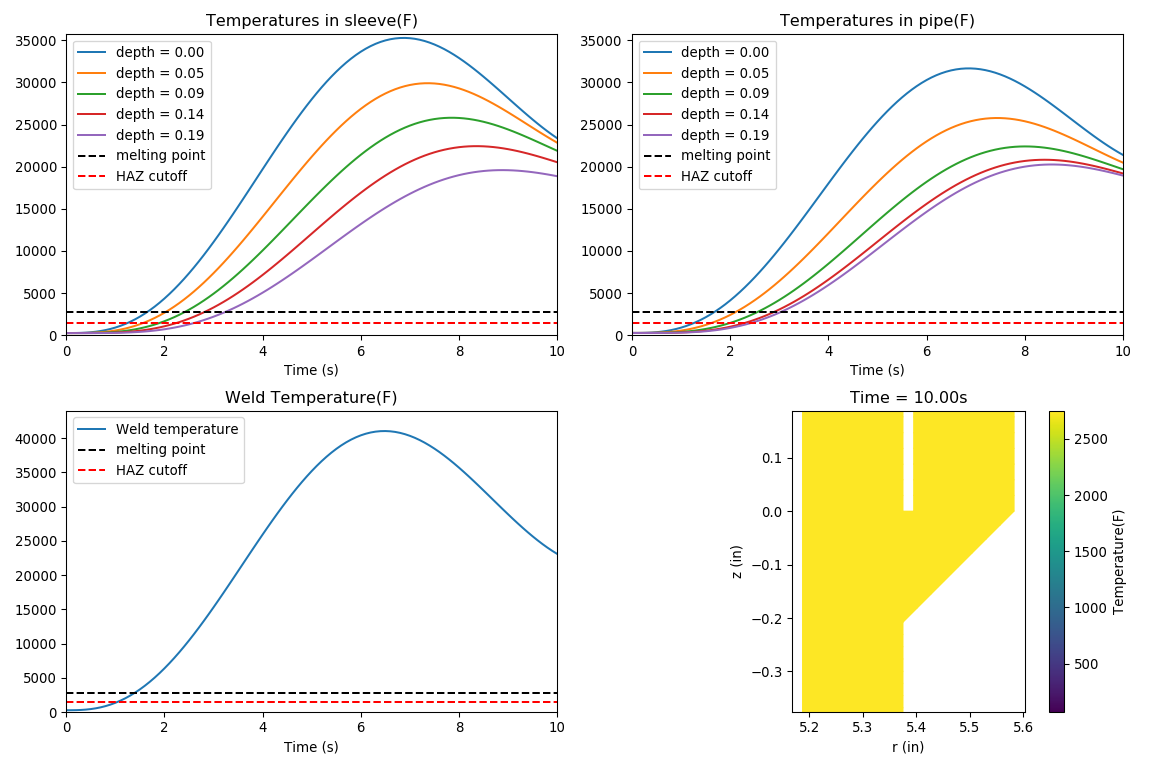
\includegraphics[width=12cm]{old_model.png}
\caption{With the given heat source density, the temperature of the weld and the substrates exceed 10 times the melting point of steel}
\label{fig2}
\end{figure}

\textbf{For the rest of the report, I used a maximum heating rate $f_{max}$ of $270~ BTU/s-in^3$.}


\subsection{Heat affected zone}
	The results of the model with the modified heating rate are shown in figure \ref{fig3}. The depth in figure \ref{fig3}a represents the distance of the point of temperature measurement from the weld, where the points are chosen along the centerline of the weld. The heat affected zone (HAZ) spans the entire thickness of the pipeline, assuming a cutoff of $1475 \degree F$ ($1075 K$)\autocitel{cheng2004weld} for the HAZ. The weld material heats up and reaches melting temperature within 4 seconds, while the weld pool starts forming at the pipe  and sleeve in in 5 and 4.5 seconds respectively. The depth of weld pool in the pipe is $0.06 in$. The cooling effect of the fluid in the pipeline is depicted by the difference in temperature history between the sleeve and the pipe. \\ 
	These temperature profiles can be used as an input for a microstructure model(see discussion) to estimate the possibility of cold cracking. Alternatively, the peak temperatures and the cooling time between $1500-1000 \degree F$ ($800-500 \degree C$)can be used to estimate the possibility of cold cracking \autocitel{lobanov2013formation}. 

\begin{figure}[h]
	\centering
	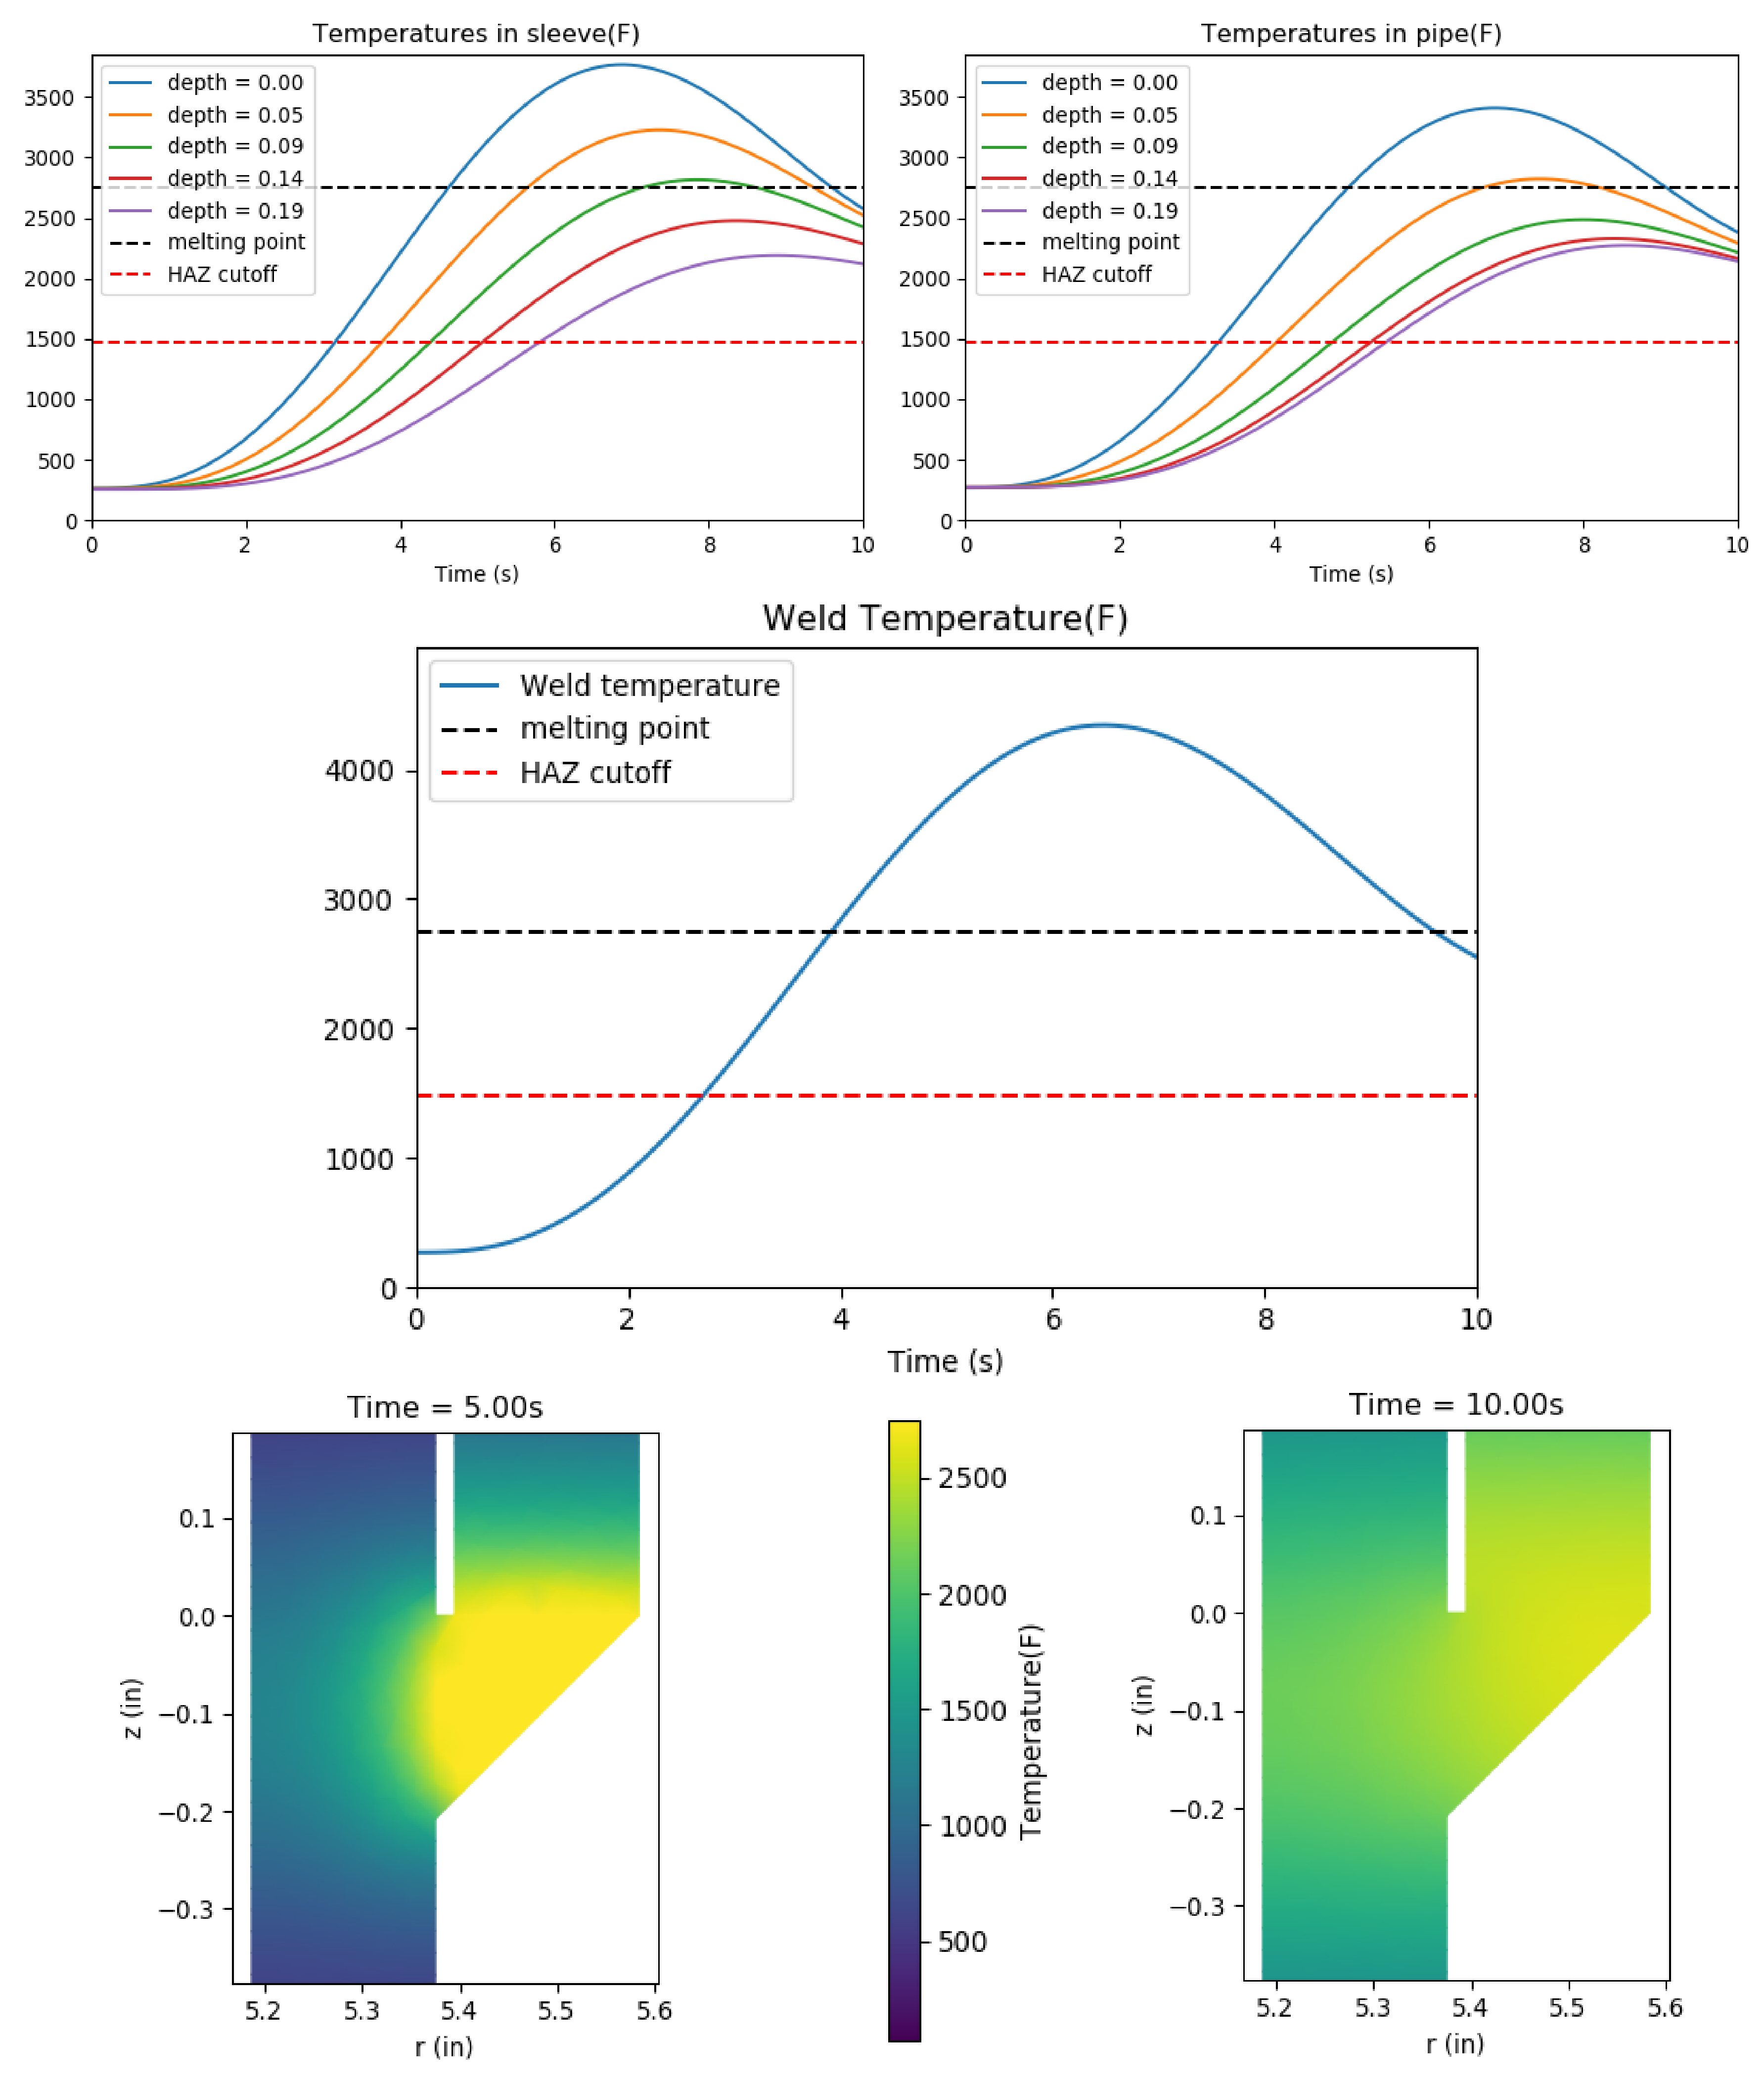
\includegraphics[width=12 cm]{linear_results.png}
	\caption{ Temperature history \textbf{a.} at different points in the sleeve and pipe and \textbf{b.} the midpoint of the weld. \textbf{c.} The temperature profile in the neighborhood of the weld at $t = 5s$ and $t = 10s$ }
	\label{fig3}
\end{figure}

\section{Discussion}
The simulation presented here has several limitations. It is based on a linear heat transfer model and does not simulate the latent heat of melting and solidification, the interface between the solid and fluid phases and the the formation of different metallurgical phases. The fluid flow in the pipes is not explicitly modeled and therefore the effect of the fluid flow on the cooling rate and the effect of heating on the fluid flow cannot be fully understood by this model. The heating of the weld element is assumed to be a volumetric heat term, while in reality welding is performed by passing a heating element over the weld zone. Finally, the assumptions of the geometry made in this model are not completely true-to-life, as the geometry of attachments to pipelines are not always symmetric around the pipe's axis. Some of these limitations will be addressed here. 

\subsection{Fluid flow modeling}
In this simulation, the heat transfer at the wall of the pipeline is modeled by means of a single constant $h_p$, which is the heat transfer coefficient of the fluid in the pipe. This kind of model is usually sufficient to understand the heat transfer in the pipe wall and the heat transfer coefficient can be changed based on the Nusselt number of the fluid flow in the pipe. There are several models available for the calculation of the Nusslet number for laminar and turbulent flows \autocitel{nagy2018basic}. This lumped parameter model can be replaced by explicit models of flow and heat transfer in the fluid using the convection-diffusion equation. However, fluid flow simulations can be computationally expensive, especially in the turbulent flow regime and therefore the lumped parameter model used here should be preferred.

Fluid flow and heat transfer in gas-fluid mixtures can be very complicated depending on the gas/fluid ratio and the inclination of the pipeline, as gravity plays an important role in the separation of the phases \autocitel{zhang2006unified}. These models can also be computationally expensive and can be replaced by heat transfer coefficients calculated based on experimental data for different gas/fluid combinations, volume fractions and pipe inclinations\autocitel{kim1999comparison}{kim2002heat}{ghajar2010importance}. 
 

\subsection{3D modeling}
 The current model is 2D axisymmetric and assumes that a cylindrical attachment is welded over the entire circumference of the pipe. As long as an attachment is placed over the entire circumference of the pipe, we can use an axisymmetric model, where the attachments geometry is replaced with a cylindrical geometry of equivalent thermal resistance. The heat flow through the sleeve/attachment in this configuration is through its contact with the weld and through its outer walls facing the atmosphere. Based on the Biot number at these two faces, a non-axisymmetric geometry can be replaced by an equivalent cylindrical geometry \autocitel{fisher1996efficient}. For attachments that do not cover the entire circumference of the pipe, like branching pipes, 3D models are more suitable\autocitel{xue2007numerical}.   


\subsection{Heat source modeling}
 In this problem, the welding heat source is modeled as a spatially uniform time-dependent power density in the entire weld area. A more widely accepted method for modeling the heat source for MIG welding assumes a double-ellipsoid geometry for the power density\autocitel{goldak1984new}. In this method, the power density is given by the sum of two Gaussian terms given by equation \ref{qfwd} in the direction of the moving weld and \ref{qbwd} in the trailing direction. In equations \ref{qfwd} and \ref{qbwd}, the weld is moving in the z direction, with the origin at the base of the weld. $Q$ is the power source density and $a$, $b$, $c_f$ and $c_r$ define the spread of the weld power in x, y and z directions. The relative power distribution in the forward and trailing directions of the weld are given by $f_f$ and $f_r$ respectively. The speed motion of the welding source is given by $v$ (equation \ref{zeta}). This heat source model is often used in simulations performed in the frame of reference moving with the welding source, and applied to a cross section of the geometry perpendicular to the welding source motion\autocitel{lindgren2006numerical}. In this case, $\zeta$ would be a function of time only. However, to make accurate predictions of the effect of parameters \autocitel{gery2005effects}, and to simulating cases of multipass welding\autocitel{deng2006numerical}, 3D models are preferred.
 
\begin{align}
q(x,y,z,t) &= \frac{6\sqrt{3}f_fQ}{abc\pi^{\frac{3}{2}}}e^{-3x^2/a^2}e^{-3y^2/a^2}e^{-3\zeta^2/c_f^2} \label{qfwd} \\
q(x,y,z,t) &= \frac{6\sqrt{3}f_bQ}{abc\pi^{\frac{3}{2}}}e^{-3x^2/a^2}e^{-3y^2/a^2}e^{-3\zeta^2/c_r^2} \label{qbwd}\\
\zeta &= z + v(\tau-t) \label{zeta}
\end{align}   


\subsection{Microstructure modeling}
	Computational thermodynamic and kinetic calculations are used to estimate the distribution of various microstructural phases such as martensite and ferrite, and the hardness of the weld and the heat affected zone. The thermodynamic models are used to calculate the free energy of the mixture as a function of the temperature and the phase composition. The free energy minimization is used to calculate the equilibrium compositions. The equilibrium reactions and the kinetics of the reactions, along with the temperature history from heat simulations are used to predict the microstructure in the heat affected zone after cooling. Some models perform heat transfer calculations separately to predict the temperatures history and use it as an input for microstructure prediction \autocitel{cheng2004weld}{mazurovsky2003phenomenological}{babu2001modeling}, while other models couple the heat transfer and microstructural calculations \autocitel{henwood1988coupled}{watt1988algorithm}{li1998computational}.   

\subsection{Modeling latent heat}
	The model presented in the previous section does not simulate the effect of change in enthalpy during melting. There are several methods of simulating the effect of enthalpy. One of the most technically sound method is to solve the Stephan problem, where the solid and fluid phases around the melt pool and heat transfer their interface is explicitly modeled \autocitel{kasuya1997stefan}. The Stephan problem can be computationally expensive and there are several simplified models, where a temperature-dependent capacitance is used to account for the enthalpy change during heating with spatial or temporal averaging \autocitel{pham1995comparison}.
	
	I chose to model total enthalpy ($H(u)$) at temperature $u$, which is a function of phase and temperature, by a smooth sigmoid function (equation \ref{enthalpy}). In equation \ref{enthalpy}, $c_{p1}$ is the specific heat due to temperature and $c_{p1}$ is the latent heat. The sigmoid function is centered around the melting point$u_{melt}$  and smoothed by the factor $a_{c_p}$. For the $n^{th}$ time step the effective specific heat is given by equation \ref{spec}, which was proposed by Morgan \textit{et al}\autocitel{morgan1978improved}. A specific heat of $106 BTU/lb$ was used. Since more accuracy is required here, a time step of $0.0001s$ was used for this simulation.  
	
\begin{align}
H(u) &= c_{p1} u + c_{p2} \frac{1}{1 + e^{-a_{c_p}(u - u_{melt})}} \label{enthalpy} \\
c_p^n &= \begin{cases}
c_{p1} \qquad \qquad \qquad if ~u^n = u^{n-1} \\
\frac{H(u^n) - H(u^{n-1})}{u^n - u^{n-1}}
 ~~~ if ~u^n \neq u^{n-1} \end{cases}\label{spec}
\end{align}    

The results for the nonlinear heat capacitance model are shown in figure 4. The temperatures predicted in this model are slightly lower than those predicted by the linear model, with a $0.04 in$ deep of the weld pool in the pipe. Even though the maximum temperatures are lower in the nonlinear model, the cooling rate in the weld is lower. This could be attributed to the lower temperature gradients near the inner wall of the pipeline.

\begin{figure}[h]
	\centering
	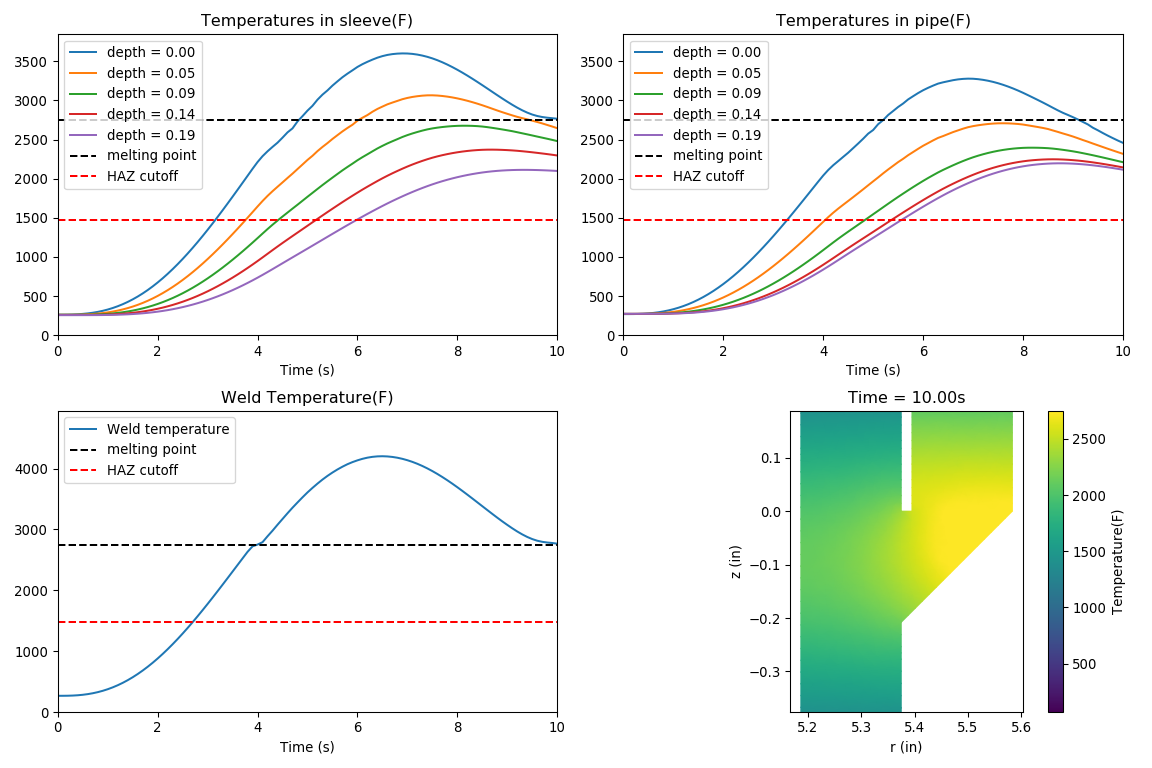
\includegraphics[width=14 cm]{nonlinear_results.png}
	\caption{ Temperature history predicted by the nonlinear model}
	\label{fig4}
\end{figure}


\end{document}